\documentclass{beamer}

\usepackage{amssymb}

\usepackage{amscd}

\usepackage[utf8]{inputenc}
\usepackage[T2A]{fontenc}
\usepackage[russian,english]{babel}
\usepackage{pgfplots}


\usepackage{tikz} 
\usetikzlibrary{arrows,matrix,patterns}

\mode<presentation>
\usetheme{Antibes}

\newtheorem{thm}{Теорема}
\newtheorem{lm}{Lemma}
\newtheorem{cl}{Следствие}
\theoremstyle{definition}
\newtheorem{df}{Definition}

\newcommand{\otime}[1]{\operatorname{O}(#1)}
\newcommand{\opoly}[1]{\otime{#1\cdot n^{\otime{1}}}}
\newcommand{\opolyone}{\otime{n^{\otime{1}}}}


\title[Задача Алкуина]{Число Алкуина графа}
\author{Павел Кунявский}
%\institute{СПбГУ}
\date{5 июня 2015}
\begin{document}

\begin{frame}
\titlepage
\begin{flushright}
руководитель: Д.\,В.~Карпов
\end{flushright}
\end{frame}

\begin{frame}
\begin{columns}[T] % align columns
\begin{column}{.73\textwidth}
Мужчине необходимо перевезти через реку волка, козу и мешок капусты. Для этого у него есть
двухместная лодка, в которую может уместиться он сам и либо волк, либо коза, либо мешок.
Можно ли перевезти всех на другую сторону реки, чтобы ни волк с козой, ни коза с мешком
капусты не оставались на одной стороне реки без присмотра?
\end{column}%
\hfill%
\begin{column}{.23\textwidth}
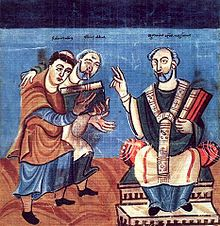
\includegraphics[scale=0.5]{Alcuin.png}
\end{column}%
\end{columns}
\end{frame}

\begin{frame}
\begin{itemize}
\item $n$ предметов
\item Лодка размера $b$
\item Произвольный граф $G$ ограничений "нельзя оставлять на одной стороне без присмотра"
\end{itemize}
\end{frame}

\begin{frame}
Формальное определение плана перевозки: набор троек $(L_1, B_1, R_1)\dots(L_s, B_s, R_s)$
\begin{itemize}
\item $L_k \sqcup B_k \sqcup R_k = V$ 
\item $|B_k| \le b$ 
\item $L_k$, $R_k$ --- независимые в $G$
\item $L_1 \sqcup B_1 = V$, $B_s \sqcup R_s = V$
\item для четных $k \ge 2$ верно $L_k = L_{k-1}$, 
\item для нечетных $k \ge 3$ выполнено $R_k = R_{k-1}$
\end{itemize}
Число Алкуина графа $AN(G)$ --- минимальный размер лодки, для которого существует план перевозки.
\end{frame}

\begin{frame}
Задача была исследована Peter Csorba, Cor A. J. Hurkens, Gerhard J. Woeginger.
Основные результаты:
\begin{lemma}
Пусть $VC(G)$ --- минимальное вершинное покрытие. 
$VC(G) \le AN(G) \le VC(G) + 1$.
\end{lemma}
\end{frame}

\begin{frame}
%\begin{columns}[T] % align columns
%\begin{column}{.73\textwidth}
\begin{thm}[структурная теорема]
$AN(G) \le b \Leftrightarrow \exists X_1, X_2, X_3, Y_1, Y_2 \subset V$
\begin{enumerate}
\item $X = X_1 \sqcup X_2 \sqcup X_3$ --- независимое.
\item $Y_1, Y_2 \subset Y = V \setminus X$, $Y_1, Y_2 \neq \varnothing$, $|Y| \le b$
\item $X_1 \sqcup Y_1$, $X_2 \sqcup Y_2$ --- независимые.
\item $|Y_1| + |Y_2| \ge |X_3|$.
\end{enumerate}
\end{thm}
\begin{cl}
Если в графе есть более одного вершинного покрытия, то $AN(G) = VC(G)$
\end{cl}
%\end{column}%i
\end{frame}
\begin{frame}
%\hfill%
%\begin{column}{.23\textwidth}
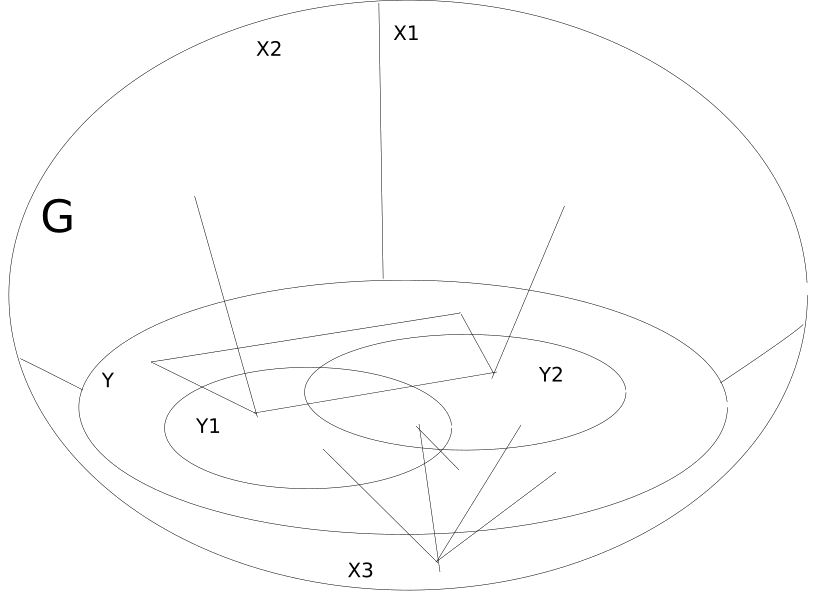
\includegraphics[scale=0.4]{structure.png}
%\end{column}%
%\end{columns}
\end{frame}


\begin{frame}
\begin{cl}
Задача о числе Алкуина может быть решена за время $\opoly{4^b}$. 
\end{cl}
Алгоритм:
\begin{itemize}
\item Найдем минимальное вершинное покрытие $Y$.
\item Если размер не $b$, то все понятно
\item Иначе переберем $4^b$ пар $Y_1, Y_2$.
\item $X_1$, $X_2$ --- все, что не связно с $Y_1, Y_2$
\item Проверили условие теоремы
\end{itemize}
\end{frame}

\begin{frame}
Оптимизация: на $Y_1, Y_2$ очень сложное условие. Надо выбрать более удачные множества для перебора.
 Заметим, что $Z = X_3 \sqcup (Y \setminus Y_2)$ --- вершинное покрытие в графе $G \setminus X_1$.
 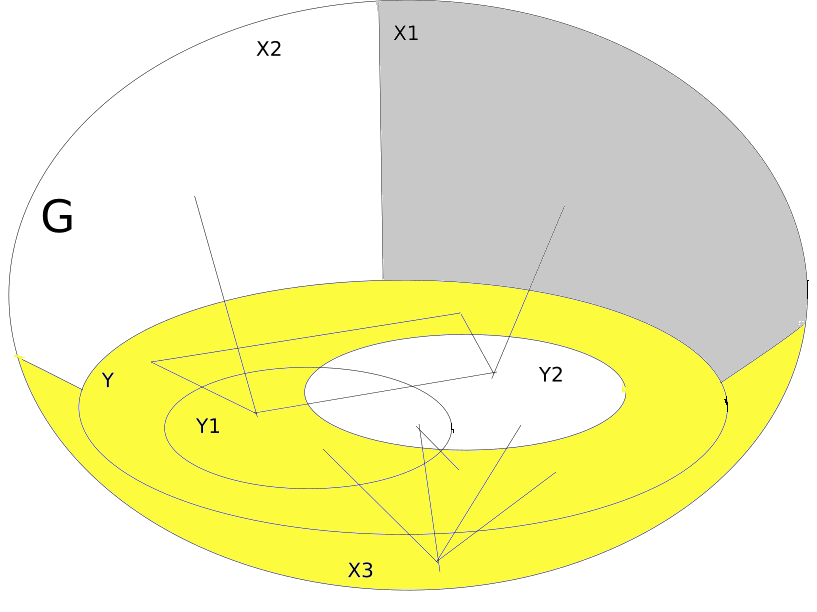
\includegraphics[scale = 0.2]{structure2.png}
\end{frame}
\begin{frame}
\begin{itemize}
\item При фиксированном $Y_1$, чтобы выполнить структурную теорему:
\item $Z$ --- вершинное покрытие $G \setminus X_1$.
\item $|Z| \le b + |Y_1|$.
\item $Y \nsubseteq Z$.
\end{itemize}
\end{frame}

\begin{frame}
\begin{thm}
Пусть задача о вершинном покрытии может быть решена
за время $\opoly{2^{\alpha VC(G)}}$
Тогда задача о числе Алкуина может быть решена за время $\opoly{2^{(1+\alpha)b}}$. 
\end{thm}
Алгоритм:
\begin{itemize}
\item Найдем минимальное вершинное покрытие $Y$
\item Если размер не $b$, то все понятно
\item Иначе переберем $2^b$ подмножеств $Y_1$
\item $X_1$ --- все, что не связно с $Y_1$
\item Найдем минимальное вершинное покрытие $Z$ в $G \setminus X_1$, не содержащее $Y$
\item Проверим условие теоремы
\end{itemize}
\end{frame}

\begin{frame}
Это решение хорошо, когда $b$ маленькое. Что делать в других случаях?
\end{frame}

\begin{frame}
Вместо частей $Y$ можно перебирать $X_1$, $X_2$.
\begin{itemize}
\item Пусть зафиксировано $X_1$. 
\item Тогда $Y_1$ --- максимальное независимое множество в $Y \setminus N_G(X_1)$.
\item Аналогично, если зафиксировать $X_2$ можно найти оптимальное $Y_2$.
\item Заметим, что выбор $Y_1$ и $Y_2$ независим, а значит их размеры можно максимизировать отдельно!
\end{itemize}
\end{frame}

\begin{frame}
Для $S \subset X$ определим $w(S)$, как размер максимального независимого множества в $Y \setminus N_G(S)$.
Тогда задача свелась к следующей:
\begin{itemize}
\item Найти $X_1, X_2 \subset X$
\item $X_1 \cap X_2 = \varnothing$
\item $w(X_1), w(X_2) > 0$
\item $w(X_1) + w(X_2) \ge n - b - |X_1| - |X_2|$
\end{itemize}
\end{frame}

\begin{frame}
\begin{itemize}
\item Задача распадается на две части. Вычисление весов и поиск оптимальной пары $X_1, X_2$.
\item Пусть задачу о независимом множестве можно решить за время $\opoly{2^{\beta n}}$.
Тогда вычислить веса можно за время $\opoly{2^{n - b + \beta b}}$, вычислив его независимо для каждого
подмножества $X$.
\item Кроме того, вычислить веса можно за время ${\opoly{2^b}}$ c помощью динамического программирования.
\end{itemize}
\end{frame}

\newcommand{\down}[1]{\left\lceil#1\right\rceil}
\newcommand{\ylog}{\down{\log{2|Y|}}}

\begin{frame}
Для поиска оптимальной пары $X_1, X_2$ определим несколько вспомогательных величин
\begin{itemize}
\item<1-> $bit(A) = \sum\limits_{k \in A}{2^k}$
\item<1-> $D(A, k) = bit(A) + 2^{|X|}\cdot k + 2^{|X| + \ylog} |A|$
\item<2-> $D(X_1, k_1) + D(X_2, k_2) = D(X_1 \sqcup X_2, k_1 + k_2)$, если $X_1$
и $X_2$ не пересекаются
\item<2-> $D(X_1, k_1) + D(X_2, k_2)$ не представимо в виде 
$D(S, s)$, если они пересекаются.
\item<2-> Таким образом, надо найти пару, $X_1, X_2$, такую, что
$D(X_1, w(X_1)) + D(X_2, w(X_2))$ представим в виде $D(S,s)$
при этом $s + |S|$ максимально.
\end{itemize}
\end{frame}

\begin{frame}
\begin{itemize}
\item Если найти все значения которые принимают $D(X_1, w(X_1)) + D(X_2, w(X_2))$,
    то задачу можно решить за $\opoly{2^{n-b}}$.
\item Рассмотрим многочлен $P(z) = \sum\limits_{\substack{A \subset X \\ w(A) > 0}}{z^{D(A, w(A))}}$
\item Все возможные значения $D(X_1, w(X_1)) + D(X_2, w(X_2))$ --- это в точности
степени мономов $P^2$. $P^2$ можно вычислить за время $\opoly{2^{n-b}}$.
\end{itemize}
\end{frame}

\begin{frame}
\begin{thm}
Задача проверки существования плана перевозки на графе размера $n$ с лодкой размера $b$
может быть решена за время $\opoly{\min(2^{(1 + \alpha) b}, 2^{n - b + \beta b}, 2^{n - b} + 2^b)}$
\end{thm}
\begin{thm}
Задача проверки существования плана перевозки на графе размера $n$
может быть решена за время $\opoly{2^{max({\frac{1 + \alpha}{2+\alpha}}, \frac{1}{2 - \beta})n}}$
\end{thm}
\end{frame}


\def\alphaval{0.2766}
\def\betavalold{0.2632}
\def\betavalnew{0.2625}
\def\betaval{\betavalold}

\begin{frame}
\pgfmathparse{(1 + \alphaval)/(2+\alphaval))+0.00007} %hack for rouning
\edef\maxfirst{\pgfmathresult}
\pgfmathparse{1/(2 - \betaval)}
\edef\maxsecond{\pgfmathresult}
\begin{thm}
Задача Алкуина на графе размера $n$
может быть решена за время 
\pgfmathparse{max(\maxfirst, \maxsecond)}
\pgfmathparse{2^(max(\maxfirst, \maxsecond))+ 0.00001} %hack for rouning
$\opoly{\pgfmathresult ^{ n}}$
\end{thm}

\begin{tikzpicture}[scale=0.9]
\begin{axis}[
    axis lines = left,
    xlabel = $\frac{b}{n}$,
    ylabel = основание экспоненты,
]
%Below the red parabola is defined
\addplot [
    domain=0:1, 
    samples=100, 
    color=red,
    dashed
]
{(2)^((1 + \alphaval) * x)};

\addplot [
    domain=0:1, 
    samples=1000, 
    color=blue,
    dashed
]
{max((2)^(x), (2)^(1 - x))};

\addplot [
    domain=0:1, 
    samples=100, 
    color=green,
    dashed
]
{(2)^(1 - x + \betaval * x)};

\addplot [
    domain=0:1, 
    samples=100, 
    color=black,
]
{min((2)^(1 - x + \betaval * x), max((2)^(x), (2)^(1 - x)), (2)^((1 + \alphaval) * x)};


\end{axis}
\end{tikzpicture}

\end{frame}

\begin{frame}
\titlepage
\begin{flushright}
руководитель: Д.\,В.~Карпов
\end{flushright}
\end{frame}

\end{document}
